\documentclass[12pt]{article}

%************* Package definitions ************************
\usepackage{graphicx}
\usepackage[utf8]{inputenc}
\usepackage[colorlinks=true,urlcolor=blue,linkcolor=blue]{hyperref}
\usepackage[sc]{mathpazo}
\usepackage[top=2cm, bottom=2cm, left=2cm, right=2cm]{geometry}
%\documentclass[english]{article}
\usepackage[T1]{fontenc}
%\usepackage[latin9]{inputenc}
\usepackage{amsmath}
\usepackage{amssymb}
\usepackage{stackrel}
\usepackage[francais]{babel}
\linespread{1.2}

%************* End of package definition ******************

\title{\textbf{Implémentation du jeu de Ngay intelligent}}
\author{\Large {GUY MBEREBE GUIDONA}\\
		\Large {OUMAR DJIME RATOU}}
\date{\today}
\begin{document}
	\pagenumbering{arabic}
	\maketitle
	\hrule
	\begin{center}
		\section*{Introduction}
	\end{center}
\noindent Le Ngay est un jeu à pions que plusieurs joueurs font circuler dans le sens trigonométrique dans deux rangées de cinq trous chacune. Il est semblable à l’awalé de l’Afrique occidentale. Cependant, il est beaucoup plus élaboré et complexe. Ainsi, dans le cadre du cours d’intelligence artificielle, il est question pour nous d’implémenter une version de ce jeu (pour cinq joueurs) et en appliquant des notions vues en cours comme celui d’un agent, les réseaux de neurones, l’apprentissage machine et bien d’autre. Nous voyons ainsi que nous essayons d’implémenter une version intelligente de ce que dans le quelle un ou plusieurs joueurs ferons face à la machine pour un match sans merci.
	\newpage
	\section{Présentation du jeu de Ngay}
\noindent Le Ngay utilise un tableau de 10 cases, qui sont creusées dans le sol ou dans le sable. Les 10 cases sont divisées en deux rangées de 5.
Le nombre de pions utilisés est de 50.\\

\begin{figure}[h!]
\begin{center}
	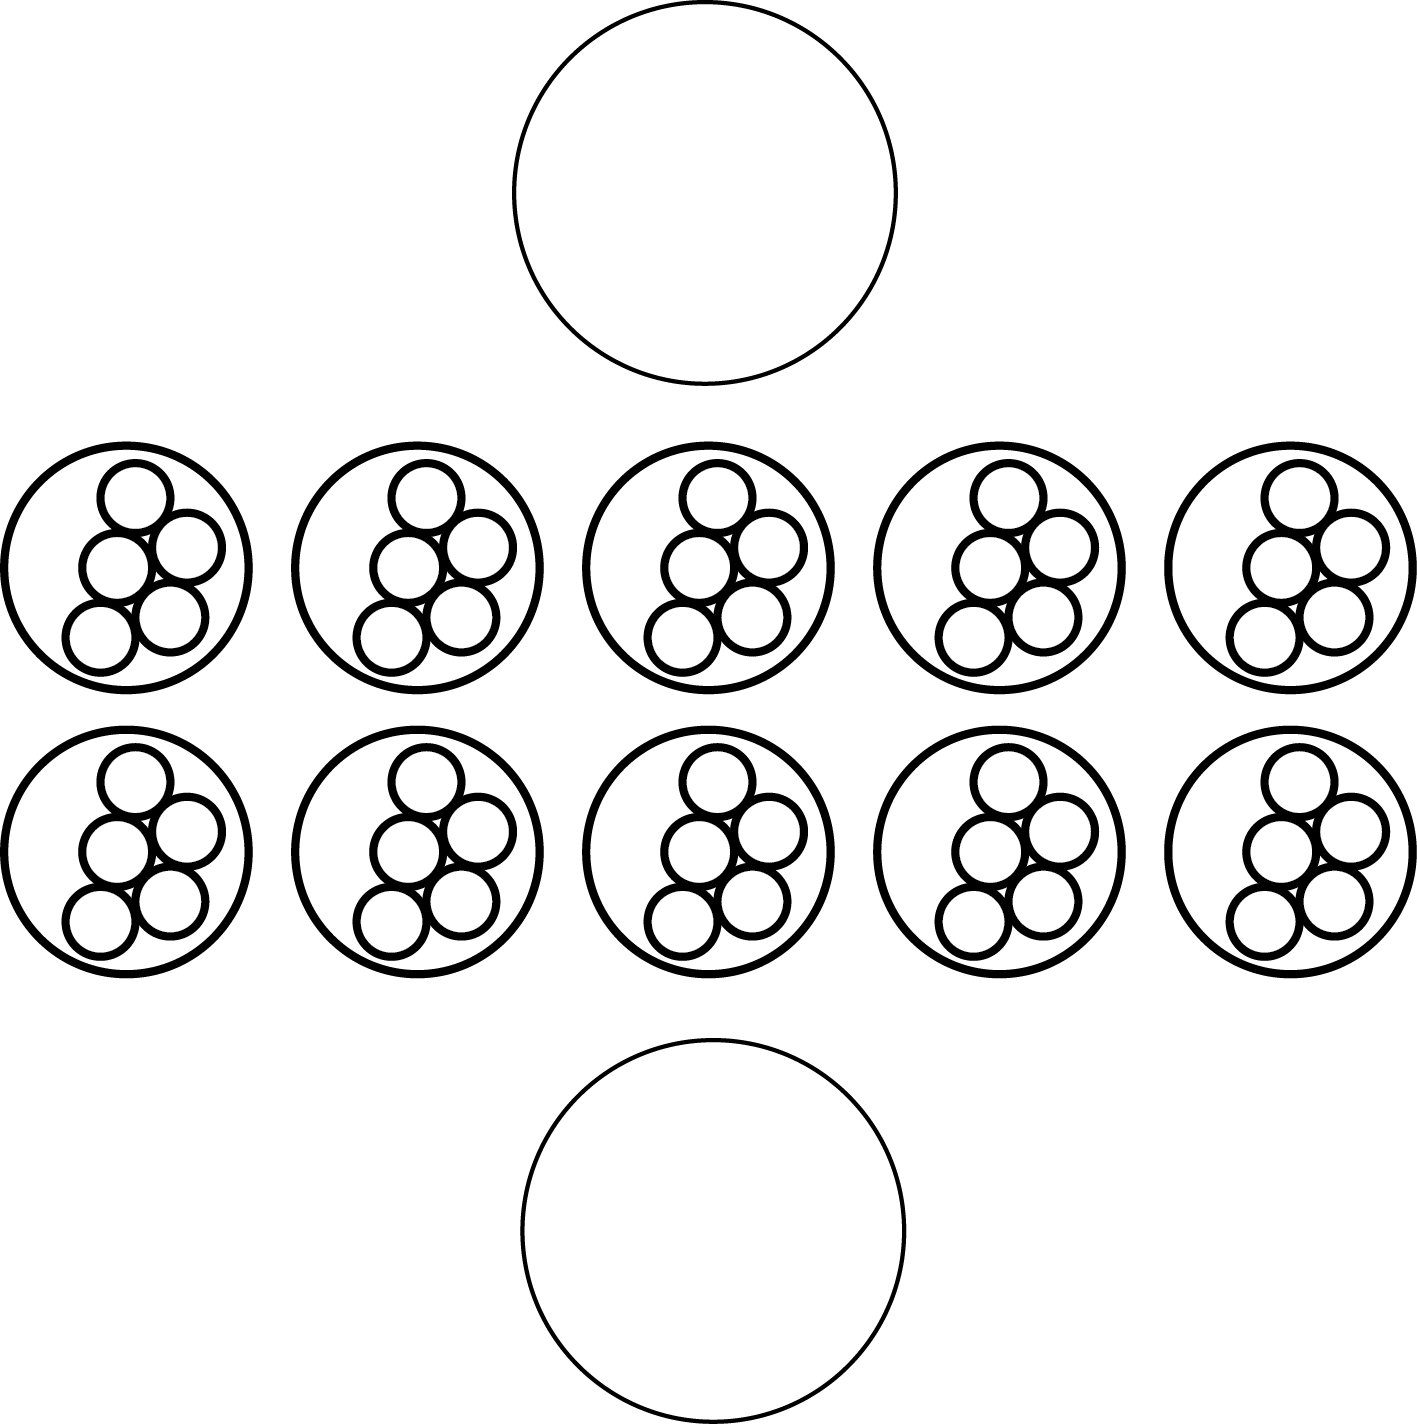
\includegraphics[scale=0.5]{images/ngay-platform}
\end{center}
\caption{Diagramme du tableau de jeu du Ngay}
\end{figure}
%Diagramme du tableau de jeu du Ngay.

\noindent Le Ngay se joue à plusieurs. Le nombre idéal de joueurs étant de 2, et la maximum 10. En présence de plusieurs joueurs, on procède, au début, à la distribution des trous. Pendant un jeu, les propriétaires ne changent pas de trous. C’est à la fin d’une séance que l’appartenance des trous aux propriétaires est constatée, afin de réajuster les nouvelles répartitions selon les pions gagnes par les uns et les autres. Le jeu lui-même est une séquence de séances. Le jeu se termine quand un seul joueur gagne tous les trous de ces adversaires. 

	\subsection{Le but du Ngay}
\noindent Le but principal du Ngay est de prendre le plus de pions possible (gagner) de ces adversaires qui initialement n’appartient à personne. Les différents types de prises seront présenter dans les sections suivantes.\\
Une personne est considérée comme gagnant lorsqu’il a gagné tous ou au moins 48 pions pour ainsi occuper tous les trous du tableau de jeu. Pour être considéré comme propriétaire légitime d’un trou, il faut y mettre au moins 3 pions sinon, elle passera à un autre.

	\subsection{Les prises dans le Ngay}
\noindent Les prises dans le Ngay sont divisées en deux (2) types. Les gains simples et les gains cumulatifs. Ces deux types de gains on a la base un même principe celui qu’on gagne qu’un nombre pair de pions en dessous de cinq (5) et que cela peut se faire dans n’importe quelles cases. 
Pour faire plus simple, les gains cumulatifs sont en fait une suite de gains simple mais dans ce cas de figure le cumule des pions pairs en dressât de 5 ne doit pas dépasser les angles de la rangée opposée. \\

	\begin{table}[h!]
		\begin{center}
		\caption{Résumé de prises}
		\begin{tabular}{|c|c|p{8cm}|}
		\hline
		 & Gain simple & Gain cumulatif\\
		\hline
		Prises & 2 ou 4 & 2 ou 4 avec les trous consécutifs répondant aux mêmes conditions\\
		\hline
		\end{tabular}
		\end{center}
	\end{table}
	
\end{document}